\subsection{GNNs for Atomic Simulations}
\subsubsection{General}
\subsubsection{Dimenet and Dimenet++}
Graph neural networks has been applied in the fields of molecular simulations. A molecule is uniquely defined by the atomic numbers $\boldsymbol{z}=\left\{z_{1}, \ldots, z_{N}\right\}$ and positions $ \boldsymbol{X}=\left\{\boldsymbol{x}_{1}, \ldots, \boldsymbol{x}_{N}\right\}$. The prediction task can be written as $f_{\theta}:\{\boldsymbol{X}, \boldsymbol{z}\} \rightarrow \mathbb{R}$, where the model outputs for example energy of the molecule. However, vanilla graph neural networks only depend on pairwise distances while ignore directional information. In order to improve the expressiveness of model, Dimenet\cite*{DBLP:journals/corr/abs-2003-03123} encodes directional information in the message embedding while keeping the network invariant to translation, rotation, and inversion of the molecule\cite*{DBLP:journals/corr/abs-2003-03123}.\\
The central idea of Dimenet is directional message embedding. For general GNNs, the atom embeddings $h_i$ are updated in each layer in the following way:\\
\begin{equation}
    \boldsymbol{h}_{i}^{(l+1)}=f_{\text {update }}\left(\boldsymbol{h}_{i}^{(l)}, \sum_{j \in \mathcal{N}_{i}} f_{\text {int }}\left(\boldsymbol{h}_{j}^{(l)}, \boldsymbol{e}_{(i j)}^{(l)}\right)\right)
\end{equation}
Where the edge embedding $\boldsymbol{e}_{(i j)}^{(l)}$ usually only depend on distance $d_{ij}$ between atom i and atom j, which limits their ability to model energy that is linked to bond angles.\\
Dimenet encodes the angle $\alpha_{(k j, j i)}=\angle \boldsymbol{x}_{k} \boldsymbol{x}_{j} \boldsymbol{x}_{i}$ and interatomic distance $d_{kj}$ in $\boldsymbol{a}_{\mathrm{SBF}}^{(k j, j i)} \in \mathbb{R}^{N_{\mathrm{SHBF}} \cdot N_{\mathrm{SRBF}}}$ which is based
on spherical Bessel functions and spherical harmonics. It also encodes $d_{ji}$ solely in $\boldsymbol{e}_{\mathrm{RBF}}^{(j i)}$ which is radial basis function.  The edge embedding is replaced by directional message embeddings $m_{ij}$. That is to say, the message passed from atom i to atom j is different from that from atom j to atom i. Dimenet updates $m_{ji}$ by aggregating all incoming edges from neighbors of atom j except for from atom i. The scheme is illustrated in figure 1 and by the following equation:
\begin{equation}
    \boldsymbol{m}_{j i}^{(l+1)}=f_{\text {update }}\left(\boldsymbol{m}_{j i}^{(l)}, \sum_{k \in \mathcal{N}_{j} \backslash\{i\}} f_{\text {int }}\left(\boldsymbol{m}_{k j}^{(l)}, \boldsymbol{e}_{\mathrm{RBF}}^{(j i)}, \boldsymbol{a}_{\mathrm{SBF}}^{(k j, j i)}\right)\right)
\end{equation}
In this way, the model is enabled to learn the angular potential energy. By encoding angular information into model, they also made the model more expressive.\\
\begin{figure}
    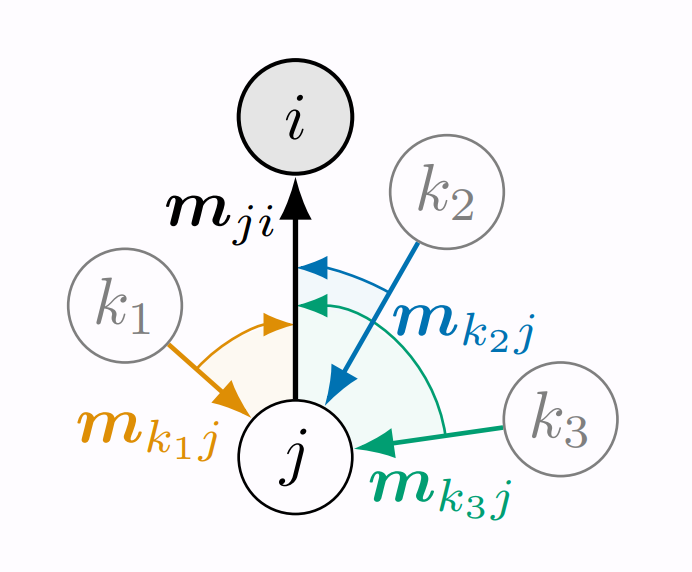
\includegraphics[width=180mm]{dimenetMS.png}
    \caption{Aggregation
    scheme for message
    embeddings. \cite*{DBLP:journals/corr/abs-2003-03123}}
  \end{figure}
The architecture of Dimenet can be illustrated in figure 2. The embedding block takes $\boldsymbol{e}_{\mathrm{RBF}}^{(j i)}$ and atomic numbers $z$ as input and outputs the initial message embeddings. The first interation block takes the initial message embedding $m_{ij}^{(1)}$ and $\boldsymbol{e}_{\mathrm{RBF}}^{(j i)}$, $\boldsymbol{a}_{\mathrm{SBF}}^{(k j, j i)}$ as input and outputs the updated message embeddings $m_{ij}^{(2)}$ for the next interation block. there are 6 interation blocks in total. Each layer including embedding block output the node embedding of their layer by aggregating message embedding coming into the atom. These node embedings are aggregated globally to output molecule level features like energy.\\
\begin{figure}
    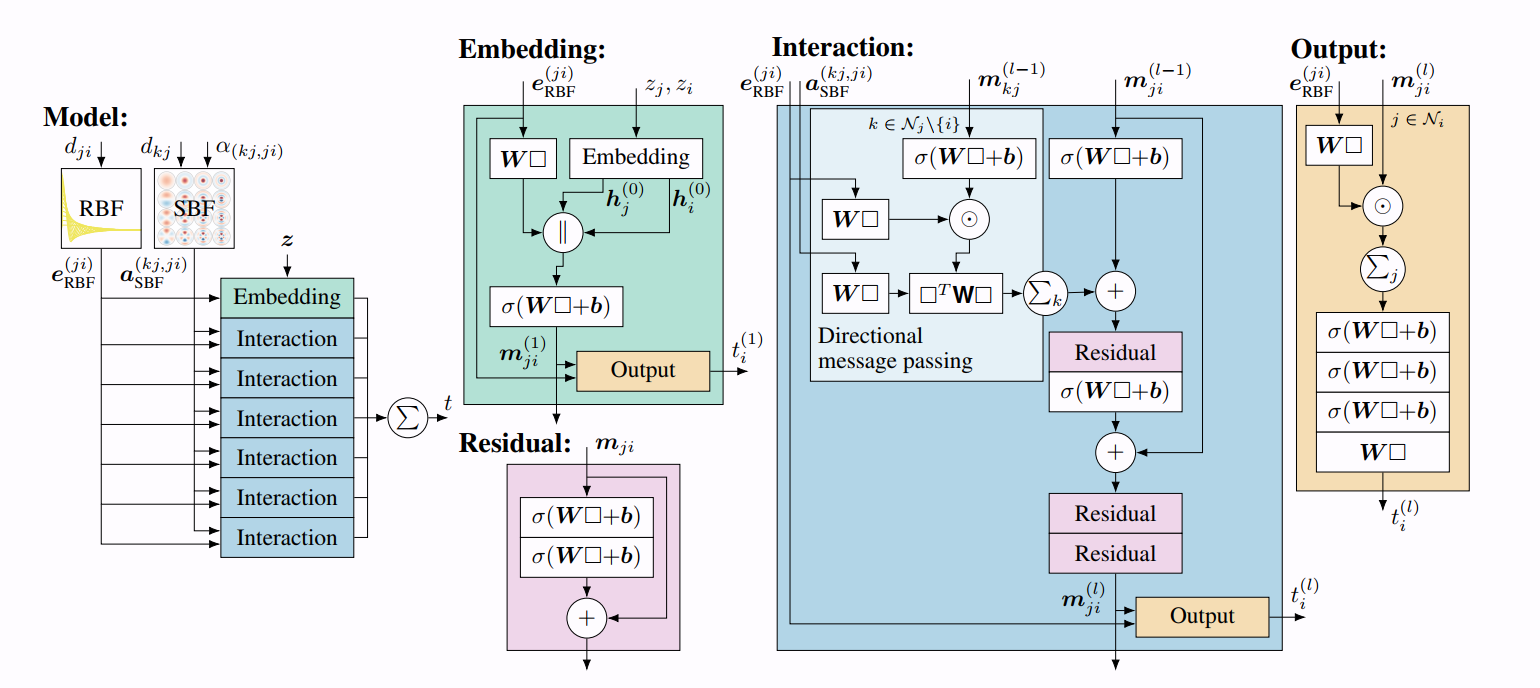
\includegraphics[width=180mm]{DimenetArch.png}
    \caption{The DimeNet architecture \cite*{DBLP:journals/corr/abs-2003-03123}}
  \end{figure}
Dimenet++ is an upgrated version of Dimenet that increases the efficiency of training without compensating the quality of results. These improvements includes: \\
\begin{itemize}
    \item replaced a bilinear layer in directional message passing block by a simplier Hadamard product and added multilayer perceptrons for the basis representations.
    \item downproject the embeddings into lower dimensions in computation-intensive parts of the model and upproject them back to the original dimensions after those layers.
    \item used 4 interation layers instead of 6. 
\end{itemize}

\begin{figure}
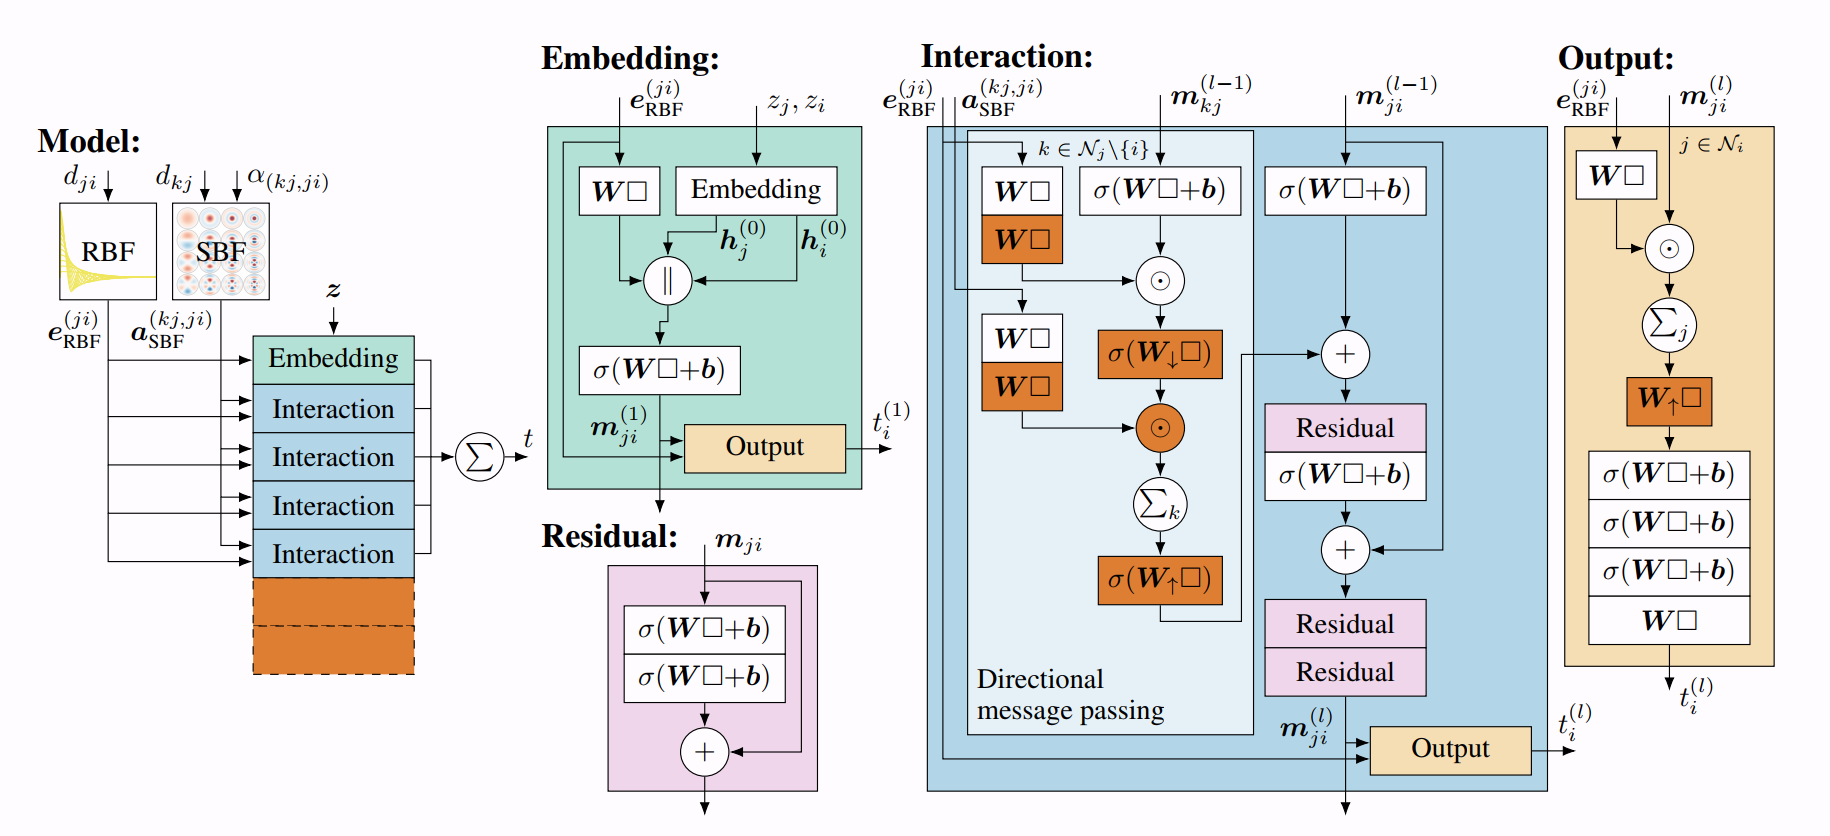
\includegraphics[width=180mm]{dimenet++.png}
\caption{The DimeNet++ architecture \cite*{https://doi.org/10.48550/arxiv.2003.03123}}
\end{figure}

